\chapter{Cordes fermées, condition d’appariement des niveaux et dualité}

\lectureoverview{Une corde fermée porte des ondes indépendantes dans ses deux directions intrinsèques. La quantification de ces ondes semble d’abord doubler le photon de la corde ouverte, mais l’invariance par translation de l’origine de la coordonnée de la corde élimine les états qui ne se propagent que dans un seul sens. Le premier niveau qui subsiste contient une particule sans masse de spin 2. La même idée de changement de description ouvre alors une question plus vaste : lorsque les couplages varient, qu’est-ce qui fait d’un objet un constituant fondamental ?}

\section{Un générateur en réserve}

Avant de dessiner une corde fermée, retrouvons un résultat de mécanique analytique. Supposons que
\begin{equation}
  L=L(q_i,\dot q_i),
\end{equation}
et définissons le moment conjugué à \(q_i\) par
\begin{equation}
  p_i=\frac{\partial L}{\partial\dot q_i}.
\end{equation}
Une transformation continue infinitésimale s’écrit
\begin{equation}
  \delta q_i=\epsilon f_i(q),
  \label{eq:l04-infinitesimal-transformation}
\end{equation}
où \(\epsilon\) est un petit paramètre. Si cette transformation est une symétrie, le théorème de Noether fournit une charge conservée. Le déplacement de la coordonnée, rapporté au paramètre commun, donne le générateur
\begin{equation}
  Q=\sum_i p_i f_i(q)
   =\frac{1}{\epsilon}\sum_i p_i\,\delta q_i.
  \label{eq:l04-noether-charge}
\end{equation}
En mécanique quantique, \(Q\) est l’opérateur qui engendre la transformation infinitésimale correspondante.

Une rotation dans le plan \(xy\) en est l’exemple usuel. Pour un choix donné de l’orientation,
\begin{equation}
  \delta x=\epsilon y,
  \qquad
  \delta y=-\epsilon x,
\end{equation}
et \eqref{eq:l04-noether-charge} devient le moment cinétique, au signe près, qui dépend du même choix. Cet exemple précis importe peu. Ce qui compte, c’est le schéma : le moment conjugué contracté avec le déplacement infinitésimal donne le générateur.

\begin{figure}[H]
  \centering
  \includegraphics[width=0.76\textwidth]{lecture_04_figure_01.png}
  \caption{Le moment canonique et le générateur de Noether gardés en réserve pour la translation ultérieure de la coordonnée de la corde fermée.}
  \lectureframe{00:05:00}
  \label{fig:l04-noether-board}
\end{figure}

Nous rencontrerons bientôt une symétrie dont la coordonnée n’est pas un point de l’espace ordinaire, mais l’étiquette des points le long d’une corde. L’équation \eqref{eq:l04-noether-charge} est présentée ici en vue de cette application.

\section{Une coordonnée autour d’une boucle}

Une corde fermée n’a pas d’extrémités. Choisissons un paramètre
\begin{equation}
  0\leq \sigma<2\pi
\end{equation}
et marquons, pour l’instant, un point comme étant \(\sigma=0\). Le point à mi-parcours est \(\sigma=\pi\) ; ceux situés au quart et aux trois quarts du tour sont \(\pi/2\) et \(3\pi/2\). Ce repère fixe une convention de coordonnée, mais ne correspond pas encore à une caractéristique physique.

\begin{figure}[H]
  \centering
  \begin{minipage}[t]{0.58\textwidth}
    \centering
    \includegraphics[width=\textwidth]{lecture_04_figure_02.png}
    \par\smallskip\footnotesize (a) La boucle marquée au tableau.
  \end{minipage}\hfill
  \begin{minipage}[t]{0.37\textwidth}
    \centering
    \begin{adjustbox}{max width=\linewidth}
    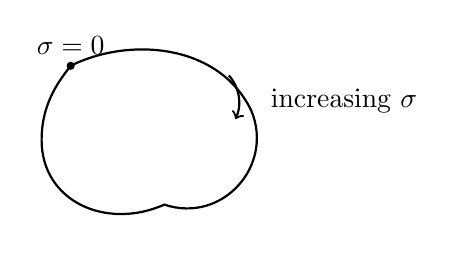
\begin{tikzpicture}[scale=0.82]
      \draw[thick]
        (0.1,1.1)
        .. controls (1.0,1.55) and (2.4,1.45) .. (2.9,0.4)
        .. controls (3.25,-0.45) and (2.45,-1.35) .. (1.55,-1.05)
        .. controls (0.65,-1.45) and (-0.35,-1.0) .. (-0.35,-0.05)
        .. controls (-0.35,0.55) and (-0.05,0.9) .. (0.1,1.1);
      \fill (0.1,1.1) circle (1.8pt);
      \node[above] at (0.1,1.12) {\(\sigma=0\)};
      \draw[->,thick] (2.55,0.95) arc[start angle=42,end angle=-25,radius=0.62];
      \node[right] at (3.05,0.55) {increasing \(\sigma\)};
    \end{tikzpicture}
    \end{adjustbox}
    \par\smallskip\footnotesize (b) L’orientation intrinsèque.
  \end{minipage}
  \caption{Un point est marqué pour définir l’origine, et une flèche fixe le sens dans lequel \(\sigma\) augmente.}
  \lectureframe{00:06:48}
  \label{fig:l04-closed-string-origin}
\end{figure}

La flèche le long de la boucle indique une orientation \emph{intrinsèque}. Il ne faut pas la confondre avec un mouvement dans le sens horaire ou antihoraire dans le plan \(xy\). Imaginons qu’on soulève du tableau un élastique marqué, qu’on le retourne et qu’on le repose. Son sens horaire apparent s’inverse, mais l’ordre de ses marques intrinsèques reste le même. Quand \(\sigma\) augmente, \(\sigma\) augmente toujours.

Cette distinction détermine le sens des mots « vers la droite » et « vers la gauche » appliqués aux ondes. Dans ce chapitre, une perturbation se propage vers la droite si elle va dans le sens des \(\sigma\) croissants, et vers la gauche si elle va dans le sens des \(\sigma\) décroissants. Ces appellations ne disent rien du sens dans lequel la perturbation semble se déplacer dans la pièce.

L’orientation jouait un rôle concret dans le modèle originel des cordes hadroniques. La rupture d’un tube de flux orienté produit un quark à une extrémité et un antiquark à l’autre ; la flèche intrinsèque distingue les deux extrémités. On peut aussi construire des théories des cordes non orientées, mais, pour l’instant, nous conservons la flèche et les deux sens le long de celle-ci.

\section{Périodicité et ondes progressives}

Soient \(X(\sigma,\tau)\) et \(Y(\sigma,\tau)\) deux coordonnées transversales de la corde, où \(\tau\) désigne le temps. Les éventuelles autres coordonnées transversales se traitent exactement de la même façon. Comme \(\sigma=0\) et \(\sigma=2\pi\) repèrent le même point,
\begin{equation}
  X(\sigma+2\pi,\tau)=X(\sigma,\tau),
  \qquad
  Y(\sigma+2\pi,\tau)=Y(\sigma,\tau).
  \label{eq:l04-periodicity}
\end{equation}

\begin{figure}[H]
  \centering
  \includegraphics[width=0.76\textwidth]{lecture_04_figure_03.png}
  \caption{Conditions aux limites périodiques pour les deux coordonnées transversales.}
  \lectureframe{00:12:40}
  \label{fig:l04-periodicity-board}
\end{figure}

Une déformation localisée peut donc circuler indéfiniment. Lorsqu’elle atteint \(2\pi\), elle réapparaît simplement en \(0\). C’est différent de ce qui se passe pour une corde ouverte, où une onde progressive atteint une extrémité et se réfléchit : une onde se propageant vers la gauche devient une onde se propageant vers la droite, et inversement. Les ondes stationnaires sont naturelles pour une corde ouverte, tandis qu’une corde fermée admet deux familles se propageant indépendamment.

\subsection{Modes de Fourier complexes}

La base la plus commode pour une fonction périodique est
\begin{equation}
  e^{in\sigma}=\cos(n\sigma)+i\sin(n\sigma),
  \qquad n\in\mathbb Z.
\end{equation}
La périodicité impose que l’indice soit entier :
\(e^{in(\sigma+2\pi)}=e^{in\sigma}\). Remplacer \(n\) par un demi-entier, par exemple, modifierait la fonction après un tour complet.

En omettant momentanément la dépendance temporelle, le développement au tableau s’écrit
\begin{align}
  X(\sigma)
  &=
  X_0+
  \sum_{n>0}X_n e^{in\sigma}
  +\sum_{n>0}X_{-n}e^{-in\sigma},
  \label{eq:l04-fourier-x}\\
  Y(\sigma)
  &=
  Y_0+
  \sum_{n>0}Y_n e^{in\sigma}
  +\sum_{n>0}Y_{-n}e^{-in\sigma}.
  \label{eq:l04-fourier-y}
\end{align}
Pour \(X\) et \(Y\) réels, les coefficients d’indice négatif sont les conjugués complexes des coefficients d’indice positif, au niveau classique. Les modes nuls \(X_0\) et \(Y_0\) indiquent la position du centre de masse ; ce sont des positions, et non des oscillations internes.

\begin{figure}[H]
  \centering
  \includegraphics[width=0.82\textwidth]{lecture_04_figure_04.png}
  \caption{Les termes d’indices positif et négatif du développement de Fourier périodique, suivis du mode nul.}
  \lectureframe{00:20:00}
  \label{fig:l04-fourier-board}
\end{figure}

\begin{classroomqa}
\audiencequestion{Si ce sont des ondes en mouvement, où est la coordonnée temporelle ?\lecturetimestamp{00:19:05}}
\lecturerresponse{Elle a simplement été omise dans la notation au tableau. Une solution propagative comporte une phase qui dépend à la fois de \(\sigma\) et de \(\tau\). Avec la convention utilisée ci-dessous, une famille comporte le facteur \(e^{-in(\tau-\sigma)}\) et l’autre le facteur \(e^{-in(\tau+\sigma)}\).}
\end{classroomqa}

C’est donc la phase complète, et non le signe de \(n\) dans un facteur de Fourier purement spatial pris isolément, qui détermine la propagation. On peut écrire
\begin{equation}
  X(\sigma,\tau)=X_R(\tau-\sigma)+X_L(\tau+\sigma),
  \label{eq:l04-chiral-solution}
\end{equation}
et, de même, pour \(Y\). La désignation de l’une des familles par \(R\) plutôt que \(L\) relève d’une convention ; le fait invariant est qu’il existe deux sens de propagation opposés le long du cercle \(\sigma\).\editorialnote{À un instant donné, le facteur \(e^{in\sigma}\) ne suffit pas à lui seul à définir une onde en mouvement. La propagation n’est déterminée qu’une fois la phase temporelle précisée.}

\section{Énergie dans les deux sens de propagation}

La dynamique locale est la même que pour la corde ouverte. Dans la normalisation simplifiée utilisée ici,
\begin{equation}
  L\propto
  \int_0^{2\pi}d\sigma\,
  \left[
    \dot X^2-X'^2+\dot Y^2-Y'^2
  \right],
  \label{eq:l04-string-lagrangian}
\end{equation}
où un point désigne \(\partial_\tau\) et une prime désigne \(\partial_\sigma\). L’énergie comporte un signe plus entre les termes cinétique et élastique :
\begin{equation}
  E\propto
  \int_0^{2\pi}d\sigma\,
  \left[
    \dot X^2+X'^2+\dot Y^2+Y'^2
  \right].
  \label{eq:l04-string-energy}
\end{equation}
Pour chacune des deux coordonnées transversales,
\begin{equation}
  \dot X^2+X'^2
  =
  \frac12(\dot X+X')^2+
  \frac12(\dot X-X')^2.
  \label{eq:l04-energy-square-completion}
\end{equation}
Les termes croisés s’annulent, laissant exactement les termes cinétiques et les termes de gradient initiaux.

\begin{figure}[H]
  \centering
  \includegraphics[width=0.82\textwidth]{lecture_04_figure_05.png}
  \caption{L’énergie totale réorganisée en deux secteurs d’ondes progressives.}
  \lectureframe{00:25:10}
  \label{fig:l04-energy-board}
\end{figure}

Pour \(X_R(\tau-\sigma)\), on a \(\dot X_R=-X_R'\) ; pour \(X_L(\tau+\sigma)\), on a \(\dot X_L=X_L'\). Les deux carrés de \eqref{eq:l04-energy-square-completion} isolent ainsi les deux familles chirales. En incluant toutes les coordonnées transversales, définissons
\begin{align}
  E_L&\propto
  \frac12\int_0^{2\pi}d\sigma
  \sum_I(\dot X^I+X^{I\prime})^2,\\
  E_R&\propto
  \frac12\int_0^{2\pi}d\sigma
  \sum_I(\dot X^I-X^{I\prime})^2.
  \label{eq:l04-left-right-energies}
\end{align}
On a alors \(E=E_L+E_R\). À ce stade, les équations étant linéaires, les ondes des deux secteurs se traversent sans diffusion.

\subsection{Deux fois plus d’oscillateurs}

Le développement en série de Fourier, substitué dans \eqref{eq:l04-string-lagrangian}, transforme chaque coefficient de mode non nul en un oscillateur harmonique. Sa fréquence est proportionnelle à \(|n|\) : plus la longueur d’onde est courte, plus la fréquence et donc l’énergie d’excitation sont élevées. Contrairement à la corde ouverte, chaque fréquence positive apparaît sous la forme de deux copies qui se propagent indépendamment.

Au tableau, les opérateurs de création polarisés selon \(X\) sont notés \(a_n^+\) et \(a_{-n}^+\), et ceux qui sont polarisés selon \(Y\), \(b_n^+\) et \(b_{-n}^+\). Pour distinguer plus clairement création et sens de propagation, nous écrirons
\begin{equation}
  a_n^\dagger,\quad b_n^\dagger,
  \qquad
  \widetilde a_n^\dagger,\quad\widetilde b_n^\dagger,
  \qquad n>0.
  \label{eq:l04-oscillator-notation}
\end{equation}
Les opérateurs sans tilde et ceux avec tilde créent des excitations se propageant dans des sens opposés sur la feuille d’univers ; \(a\) et \(b\) désignent les deux polarisations transversales.

\begin{figure}[H]
  \centering
  \includegraphics[width=0.65\textwidth]{lecture_04_figure_06.png}
  \caption{La notation du tableau pour les opérateurs de création dédoublés, polarisés selon \(X\) et \(Y\).}
  \lectureframe{00:29:10}
  \label{fig:l04-oscillators-board}
\end{figure}

Si \(N_n^{(a)},N_n^{(b)}\) et leurs partenaires tildés sont des nombres d’occupation, les niveaux d’oscillation transportés dans les deux sens s’écrivent schématiquement
\begin{equation}
  \begin{aligned}
    N&=\sum_{n>0}n\bigl(N_n^{(a)}+N_n^{(b)}+\cdots\bigr),\\
    \widetilde N&=\sum_{n>0}n
      \bigl(\widetilde N_n^{(a)}+\widetilde N_n^{(b)}+\cdots\bigr).
  \end{aligned}
  \label{eq:l04-level-operators}
\end{equation}
Les points de suspension représentent les autres directions transversales.

\section{La prédiction sur le spectre qui échoue}

Rappelons le premier niveau de la corde ouverte. L’action de \(a_1^\dagger\) ou de \(b_1^\dagger\) sur l’état fondamental donne deux polarisations linéaires. Leurs combinaisons circulaires,
\begin{equation}
  c_\pm^\dagger
  =
  \frac{1}{\sqrt2}
  \left(a_1^\dagger\pm i b_1^\dagger\right),
  \label{eq:l04-open-circular}
\end{equation}
portent l’hélicité \(h=\pm1\). L’absence d’un partenaire d’hélicité nulle est la signature d’un vecteur sans masse dans cette description élémentaire à quatre dimensions.

Soit \(m_0^2\) la masse au carré de l’état fondamental de la corde fermée. Une première conjecture naïve consiste à agir une fois avec l’un des opérateurs suivants :
\begin{equation}
  a_1^\dagger,\quad b_1^\dagger,\quad
  \widetilde a_1^\dagger,\quad\widetilde b_1^\dagger.
  \label{eq:l04-naive-one-sided}
\end{equation}
Cela ressemble à deux copies du photon de la corde ouverte, une pour chaque sens de propagation. Au niveau d’énergie suivant, toutefois, la liste non restreinte ne s’organise pas en multiplets de rotation cohérents. Le problème ne se résout pas avec des règles de dénombrement plus élaborées. L’hypothèse selon laquelle tout monôme d’oscillateurs est un état physique est fausse.

\subsection{L’appariement des niveaux, d’abord posé comme règle}

La condition physique pour la corde fermée est
\begin{equation}
  N=\widetilde N,
  \qquad\text{equivalently}\qquad E_L=E_R.
  \label{eq:l04-level-matching}
\end{equation}
Pour l’instant, prenons-la comme un postulat ; nous n’en déduirons l’origine qu’après avoir vu ce qu’elle permet d’obtenir.

Chaque état de \eqref{eq:l04-naive-one-sided} porte une unité d’énergie dans un secteur et aucune dans l’autre ; ils sont donc tous exclus. Les premiers états qui subsistent comportent un oscillateur de chaque famille :
\begin{align}
  a_1^\dagger\widetilde a_1^\dagger\ket{0},
  &\qquad
  b_1^\dagger\widetilde b_1^\dagger\ket{0},
  \label{eq:l04-four-matched-a}\\
  a_1^\dagger\widetilde b_1^\dagger\ket{0},
  &\qquad
  b_1^\dagger\widetilde a_1^\dagger\ket{0}.
  \label{eq:l04-four-matched-b}
\end{align}
Ils ont une énergie totale d’oscillation de deux unités, répartie également entre les deux sens. Un opérateur de création unique \(n=2\) a la même énergie totale d’oscillation, mais ne satisfait pas \eqref{eq:l04-level-matching} ; il apporte deux unités d’un seul côté.

\begin{figure}[H]
  \centering
  \includegraphics[width=0.70\textwidth]{lecture_04_figure_07.png}
  \caption{Les quatre états du premier niveau qui satisfont à la condition d’appariement des niveaux. Le tableau utilise les indices \(1\) et \(-1\) là où \eqref{eq:l04-four-matched-a}--\eqref{eq:l04-four-matched-b} emploie les opérateurs sans tilde et avec tilde.}
  \lectureframe{00:41:05}
  \label{fig:l04-level-matched-board}
\end{figure}

\section{Un graviton au premier niveau apparié}

Plaçons les deux familles chirales dans une base circulaire :
\begin{equation}
  c_\pm^\dagger
  =\frac{a_1^\dagger\pm i b_1^\dagger}{\sqrt2},
  \qquad
  \widetilde c_\pm^\dagger
  =\frac{\widetilde a_1^\dagger\pm i\widetilde b_1^\dagger}{\sqrt2}.
  \label{eq:l04-closed-circular}
\end{equation}
Chaque facteur contribue à l’hélicité \(+1\) ou \(-1\) dans l’espace transverse ordinaire. Leurs produits donnent donc
\begin{center}\begin{tabular}{c c}\toprule
  État & Hélicité \\
  \midrule
  \(c_+^\dagger\widetilde c_+^\dagger\ket0\) & \(+2\) \\
  \(c_-^\dagger\widetilde c_-^\dagger\ket0\) & \(-2\) \\
  \(c_+^\dagger\widetilde c_-^\dagger\ket0\) & \(0\) \\
  \(c_-^\dagger\widetilde c_+^\dagger\ket0\) & \(0\) \\
  \bottomrule
\end{tabular}
\end{center}

\begin{classroomqa}
\audiencequestion{Le second facteur de polarisation circulaire doit-il provenir du secteur de propagation opposé ?\lecturetimestamp{00:43:20}}
\lecturerresponse{Oui. C’est précisément pour cette raison que la première expression écrite au tableau a été corrigée. Ici, un état physique doit associer un oscillateur se propageant vers la droite à un oscillateur se propageant vers la gauche ; sinon, la condition d’appariement des niveaux n’est pas satisfaite. Les hélicités se rapportent à la polarisation dans l’espace transverse, tandis que les deux facteurs correspondent aux sens opposés de propagation sur la feuille d’univers.}
\end{classroomqa}

\begin{figure}[H]
  \centering
  \includegraphics[width=0.82\textwidth]{lecture_04_figure_08.png}
  \caption{Les quatre produits de la base circulaire après la correction apportée au tableau, avec les hélicités \(+2,-2,0,0\).}
  \lectureframe{00:46:10}
  \label{fig:l04-helicity-board}
\end{figure}

Une particule massive de spin 2 possède cinq projections de spin,
\begin{equation}
  m=2,1,0,-1,-2.
\end{equation}
Le niveau apparié ne contient aucun partenaire \(m=\pm1\). Il ne peut donc pas former un multiplet de spin 2 massif. En revanche, une particule sans masse de spin 2 ne possède que les hélicités \(+2\) et \(-2\). Les produits de même hélicité sont exactement ces deux états : ce sont les polarisations du graviton.

Il reste deux combinaisons d’hélicité nulle. Dans les termes employés en cours, l’une est le dilaton et l’autre l’axion. Une description covariante de la corde bosonique fermée générique précise cette affirmation :
\begin{equation}
  \begin{aligned}
    \alpha_{-1}^{I}\widetilde\alpha_{-1}^{J}\ket{0;k}
    &\longrightarrow
    \underbrace{h_{IJ}}_{\text{symmetric traceless}}
    \oplus
    \underbrace{B_{IJ}}_{\text{antisymmetric}}\\
    &\hspace{2.5em}\oplus
    \underbrace{\Phi}_{\text{trace}}.
  \end{aligned}
  \label{eq:l04-massless-tensor-decomposition}
\end{equation}
Il s’agit du graviton, d’une 2-forme antisymétrique et du dilaton. En quatre dimensions, la 2-forme peut être dualisée en un pseudoscalaire de type axion, selon la terminologie adoptée dans le cours.\editorialnote{Fondamentalement, le second état d’hélicité nulle est le champ tensoriel antisymétrique \(B_{\mu\nu}\) dans le spectre générique de la corde fermée. Le qualifier d’axion correspond à sa description duale en quatre dimensions.}

À ce niveau formel, les trois champs sont sans masse. La compactification, les projections et la dynamique du fond peuvent modifier les degrés de liberté scalaires ou ceux de la 2-forme qui restent légers. Le graviton est différent : dès qu’un secteur cohérent de cordes fermées en interaction est présent, son état de spin 2 sans masse est inévitable. C’est pourquoi la gravité émerge des cordes fermées au lieu d’être ajoutée comme ingrédient distinct.

\section{Pourquoi les niveaux doivent s’apparier}

Revenons maintenant au repère en \(\sigma=0\). Est-ce une perle physique attachée à la boucle, ou simplement l’origine de notre paramètre ? Pour une corde fermée ordinaire non marquée, aucun point ne doit être privilégié. L’état quantique doit rester inchangé quand toutes les étiquettes sont translatées ensemble.

\subsection{La version discrète}

Découpons la boucle en \(M\) points ordonnés, de coordonnées transversales \((X_i,Y_i)\). Omettons temporairement \(Y_i\). La fonction d’onde dans l’espace des configurations est
\begin{equation}
  \Psi(X_1,X_2,\ldots,X_M).
\end{equation}
Changer le point désigné comme premier produit une permutation cyclique :
\begin{align}
  \Psi(X_1,X_2,\ldots,X_M)
  &=
  \Psi(X_2,\ldots,X_M,X_1)\nonumber\\
  &=
  \Psi(X_3,\ldots,X_M,X_1,X_2).
  \label{eq:l04-cyclic-wavefunction}
\end{align}
Il ne s’agit pas d’une invariance sous une permutation arbitraire. Insérer \(X_3\) entre \(X_1\) et \(X_2\), par exemple, modifie la structure des voisinages et revient à déchirer puis reconnecter la corde discrétisée. Seul le réétiquetage cyclique commun
\begin{equation}
  X_i\longrightarrow X_{i+1}\qquad(\text{mod }M)
  \label{eq:l04-discrete-shift}
\end{equation}
exprime l’absence d’une origine privilégiée.

\begin{figure}[H]
  \centering
  \includegraphics[width=0.82\textwidth]{lecture_04_figure_09.png}
  \caption{Les identités cycliques de la fonction d’onde d’une corde fermée discrétisée.}
  \lectureframe{00:56:20}
  \label{fig:l04-cyclic-board}
\end{figure}

\subsection{La version continue}

À la limite continue \(M\to\infty\), l’état est la fonctionnelle d’onde
\begin{equation*}
  \Psi[X(\sigma),Y(\sigma)].
\end{equation*}
Un réétiquetage cyclique devient
\begin{equation}
  \sigma\longrightarrow\sigma+\epsilon.
\end{equation}
L’invariance s’écrit
\begin{equation}
  \Psi[X(\sigma+\epsilon),Y(\sigma+\epsilon)]
  =
  \Psi[X(\sigma),Y(\sigma)].
  \label{eq:l04-wavefunctional-invariance}
\end{equation}

\begin{figure}[H]
  \centering
  \includegraphics[width=0.72\textwidth]{lecture_04_figure_10.png}
  \caption{La translation discrète et son expression continue pour la fonctionnelle d’onde.}
  \lectureframe{00:58:40}
  \label{fig:l04-wavefunctional-board}
\end{figure}

Au premier ordre,
\begin{equation}
  \delta X(\sigma)=\epsilon X'(\sigma),
  \qquad
  \delta Y(\sigma)=\epsilon Y'(\sigma),
  \label{eq:l04-profile-shift}
\end{equation}
à un signe global près, qui distingue une translation active du profil d’une translation passive de la coordonnée. La variation correspondante de la fonctionnelle d’onde est
\begin{equation}
  \delta\Psi
  =
  \epsilon\int_0^{2\pi}d\sigma
  \left[
    \frac{\delta\Psi}{\delta X(\sigma)}X'(\sigma)
    +
    \frac{\delta\Psi}{\delta Y(\sigma)}Y'(\sigma)
  \right].
  \label{eq:l04-functional-variation}
\end{equation}

\begin{figure}[H]
  \centering
  \includegraphics[width=0.72\textwidth]{lecture_04_figure_11.png}
  \caption{Le développement au premier ordre de l’argument translaté de la fonctionnelle d’onde.}
  \lectureframe{01:01:31}
  \label{fig:l04-functional-expansion-board}
\end{figure}

\begin{classroomqa}
\audiencequestion{La condition au premier ordre constitue-t-elle une équation distincte pour chaque valeur de \(\sigma\) ?\lecturetimestamp{01:01:30}}
\lecturerresponse{Non. La transformation translate ensemble tous les points de la corde. Il faut additionner la variation en un point à celles de tous les autres points, d’où l’intégrale sur \(\sigma\) dans l’expression continue.}
\end{classroomqa}

Dans la représentation de coordonnées,
\begin{equation}
  P_X(\sigma)=-i\frac{\delta}{\delta X(\sigma)},
  \qquad
  P_Y(\sigma)=-i\frac{\delta}{\delta Y(\sigma)}
  \label{eq:l04-functional-momenta}
\end{equation}
avec \(\hbar=1\). L’équation \eqref{eq:l04-functional-variation} est donc engendrée par
\begin{equation}
  G_\sigma=
  \int_0^{2\pi}d\sigma\,
  \left[
    P_X(\sigma)X'(\sigma)+P_Y(\sigma)Y'(\sigma)
  \right].
  \label{eq:l04-sigma-generator}
\end{equation}
On retrouve exactement le schéma de Noether \eqref{eq:l04-noether-charge} : le moment canonique multiplié par le déplacement de la coordonnée, avec une somme sur tous les degrés de liberté. Un état de corde fermée non marquée vérifie
\begin{equation}
  G_\sigma\ket{\mathrm{phys}}=0.
  \label{eq:l04-physical-generator-condition}
\end{equation}

Pour la normalisation de \eqref{eq:l04-string-lagrangian},
\(P_I\propto\dot X^I\), de sorte que la même condition s’écrit
\begin{equation}
  \int_0^{2\pi}d\sigma
  \sum_I\dot X^I X^{I\prime}=0.
  \label{eq:l04-momentum-constraint}
\end{equation}

\begin{figure}[H]
  \centering
  \includegraphics[width=0.75\textwidth]{lecture_04_figure_12.png}
  \caption{Le générateur intégré, après identification de la dérivée de la fonctionnelle d’onde au moment.}
  \lectureframe{01:05:10}
  \label{fig:l04-generator-board}
\end{figure}

\subsection{Le générateur est la différence des énergies}

La somme des deux expressions de \eqref{eq:l04-left-right-energies} est l’énergie totale. Leur différence vaut
\begin{align}
  E_L-E_R
  &\propto
  \frac12\int_0^{2\pi}d\sigma\sum_I
  \left[
    (\dot X^I+X^{I\prime})^2\right.\nonumber\\[-0.25em]
  &\hspace{7em}\left.
    -(\dot X^I-X^{I\prime})^2
  \right]\\
  &=
  2\int_0^{2\pi}d\sigma\sum_I
  \dot X^I X^{I\prime}.
  \label{eq:l04-energy-difference}
\end{align}
L’intégrale est le générateur qui doit annuler un état physique. Par conséquent,
\begin{equation}
  E_L-E_R=0,
  \qquad\text{or}\qquad
  N-\widetilde N=0.
\end{equation}
L’appariement des niveaux signifie que l’origine de la coordonnée \(\sigma\) est inobservable.

\begin{figure}[H]
  \centering
  \includegraphics[width=0.78\textwidth]{lecture_04_figure_13.png}
  \caption{La somme et la différence des énergies présentées ensemble à la fin de la dérivation de l’appariement des niveaux.}
  \lectureframe{01:06:40}
  \label{fig:l04-energy-difference-board}
\end{figure}

\begin{classroomqa}
\audiencequestion{Pourquoi les formules affichées semblent-elles placer le facteur un demi différemment ?\lecturetimestamp{01:06:28}}
\lecturerresponse{Seule la structure relative est utilisée ici. En rétablissant une normalisation globale cohérente, on retrouve le facteur un demi dans l’identité de mise sous forme de carré \eqref{eq:l04-energy-square-completion}. La somme donne l’énergie totale, tandis que la différence reste proportionnelle à \(\int d\sigma\,\dot X X'\). Son annulation, et donc l’appariement des niveaux, ne dépend pas de cette convention commune.}
\end{classroomqa}

La contrainte élimine une grande partie du spectre naïf des oscillateurs, et précisément les états qui ne formaient pas de multiplets de particules cohérents. Elle n’élimine pas le photon de la corde ouverte, car une corde ouverte ne possède pas deux secteurs indépendants en circulation soumis à cette condition propre aux boucles fermées. Pour la corde fermée, elle laisse subsister le graviton, le dilaton, l’état associé au tenseur antisymétrique ou de type axion, ainsi que les niveaux appariés supérieurs. \editorialnote{Dans la quantification covariante des cordes, l’appariement des niveaux est la condition sur le mode zéro \(L_0-\widetilde L_0=0\), qui fait partie du système de contraintes de la feuille d’univers. La dérivation présentée ici en isole l’origine intuitive : l’invariance par translation le long de la corde fermée.}

\section{Deux sens distincts de « gauche » et « droite »}

Il existe désormais deux emplois sans rapport du vocabulaire de la chiralité :
\begin{enumerate}
  \item \(X_R(\tau-\sigma)\) et \(X_L(\tau+\sigma)\) décrivent la propagation dans des sens opposés le long du cercle intrinsèque \(\sigma\).
  \item \(c_+^\dagger\) et \(c_-^\dagger\) décrivent la polarisation circulaire dans le plan transverse physique \(xy\).
\end{enumerate}
L’état du graviton qui satisfait à l’appariement des niveaux contient un oscillateur de chaque sens de propagation sur la feuille d’univers. Ces deux oscillateurs peuvent néanmoins avoir la même hélicité dans l’espace-temps, donnant \(h=+2\) ou \(h=-2\). Confondre ces deux sens de « gauche » et de « droite » donne au spectre une apparence contradictoire, alors qu’il ne l’est pas.

\section{Que signifie « fondamental » ?}

Une fois les cordes ouvertes et fermées quantifiées à ce niveau élémentaire, une question naturelle demeure : les cordes sont-elles les constituants ultimes, ou pourraient-elles elles-mêmes être faites d’autre chose ?

\begin{classroomqa}
\audiencequestion{Existe-t-il des éléments ou une raison de considérer les cordes comme les objets les plus fondamentaux, sans constituants plus petits en dessous ?\lecturetimestamp{01:10:44}}
\lecturerresponse{Il n’existe pas de réponse utile indépendante des paramètres. Les degrés de liberté qui paraissent élémentaires dans un régime peuvent devenir lourds, étendus et apparemment composites dans un autre. Il vaut mieux comprendre « fondamental » comme une indication des variables qui fournissent la description la plus utile au couplage considéré.}
\end{classroomqa}

Les charges électriques et magnétiques fournissent l’exemple le plus clair. Supposons qu’une théorie contienne une charge électrique \(e\) et une charge magnétique \(g\). La chaîne de Dirac inobservable attachée à un monopôle impose la condition
\begin{equation}
  eg=2\pi n,
  \qquad n\in\mathbb Z.
  \label{eq:l04-dirac-quantization}
\end{equation}
Pour les charges minimales, \(n=1\). Une particule chargée qui fait le tour de la chaîne de Dirac acquiert alors une phase \(e^{ieg}=1\), si bien que cette chaîne auxiliaire ne peut pas être détectée.

\begin{figure}[H]
  \centering
  \begin{minipage}[t]{0.58\textwidth}
    \centering
    \includegraphics[width=\textwidth]{lecture_04_figure_14.png}
    \par\smallskip\footnotesize (a) Quantification de Dirac au tableau.
  \end{minipage}\hfill
  \begin{minipage}[t]{0.36\textwidth}
    \centering
    \begin{adjustbox}{max width=\linewidth}
    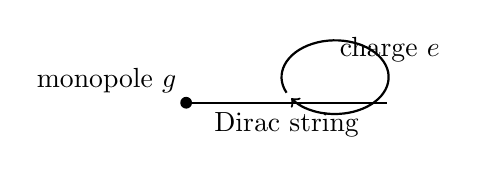
\begin{tikzpicture}[scale=0.85]
      \fill (0,0) circle (2.5pt);
      \node[above left] at (0,0) {monopole \(g\)};
      \draw[thick] (0,0) -- (3.0,0);
      \node[below] at (1.5,0) {Dirac string};
      \draw[->,thick] (1.5,0.15) arc[start angle=205,end angle=-145,
        x radius=0.8,y radius=0.55];
      \node[right] at (2.15,0.8) {charge \(e\)};
    \end{tikzpicture}
    \end{adjustbox}
    \par\smallskip\footnotesize (b) L’expérience de phase autour de la chaîne.
  \end{minipage}
  \caption{La condition de Dirac relie inversement les charges électriques et magnétiques.}
  \lectureframe{01:13:20}
  \label{fig:l04-dirac-board}
\end{figure}

Si \(e\) est petit, la théorie des perturbations usuelles en variables électriques est utile. Les diagrammes de Feynman comportant davantage de sommets électriques sont de plus en plus supprimés. Mais, d’après \eqref{eq:l04-dirac-quantization}, \(g\) est alors grand, si bien qu’un développement diagrammatique en sommets magnétiques n’est pas utile. En termes des couplages sans dimension usuels,
\begin{equation}
  \alpha_e=\frac{e^2}{4\pi},
  \qquad
  \alpha_m=\frac{g^2}{4\pi},
  \qquad
  \alpha_e\alpha_m=\frac{n^2}{4}.
  \label{eq:l04-dual-couplings}
\end{equation}
Un couplage électrique faible correspond à un couplage magnétique fort, et inversement.

Du point de vue de la description électrique, le monopôle à couplage fort paraît lui aussi compliqué. Son énergie de champ est grande ; il est habillé d’un intense nuage de fluctuations du champ de jauge et de paires virtuelles porteuses de charge magnétique. Il se comporte comme un objet lourd et étendu, qui constitue un mauvais point de départ pour un développement perturbatif électrique. Cela ne prouve pas qu’il soit moins fondamental. Cela indique que, dans ce régime, ce n’est pas la bonne variable élémentaire.

Imaginons maintenant que l’on augmente continûment \(e\). La condition de quantification impose alors que \(g\) diminue. Au voisinage du régime auto-dual, aucune des deux descriptions n’est particulièrement faiblement couplée ; au-delà, les variables magnétiques peuvent devenir plus simples et plus légères, tandis que les objets électriques deviennent fortement habillés. Le changement de la charge qualifiée d’élémentaire ne modifie pas le contenu physique de la théorie.

\subsection{La question de Wigner}

Cette ambiguïté est apparue un jour lors d’une discussion sur le caractère fondamental ou composite du boson de Higgs. Eugene Wigner demandait sans cesse ce que signifiait « composite ». Une distinction proposée reposait sur la désintégration : peut-être un objet fondamental ne peut-il pas se désintégrer, contrairement à un objet composite. Mais un atome d’hydrogène dans son état fondamental ne peut pas se désintégrer et il est manifestement composite ; le proton peut être stable alors que le neutron se désintègre, sans que cela fasse de l’un un objet élémentaire et de l’autre un objet composite au sens voulu. Chaque définition simple soulevait un nouveau contre-exemple.

Gerardus 't Hooft mit fin à la discussion en proposant ce critère opérationnel : un objet est fondamental lorsqu’il est utile de le considérer comme tel. Ce n’est pas une esquive. Cela reconnaît que le qualificatif « élémentaire » désigne les variables dans lesquelles la dynamique est simple, et que cette simplicité peut dépendre du couplage et de l’environnement.

\section{Vers la théorie M}

La théorie des cordes réalise cet échange des rôles de façon particulièrement nette. Dans un régime de paramètres, les cordes sont légères et perturbatives, tandis que les D-branes apparaissent comme de lourds objets solitoniques composites, constitués de degrés de liberté des cordes. Lorsque les paramètres changent, les D-branes peuvent devenir les objets élémentaires les plus légers, et les configurations décrites comme des cordes dans le premier régime peuvent être réinterprétées en termes de D-branes. Ce qui semblait fondamental peut devenir composite ; ce qui semblait composite peut devenir fondamental.

L’ancienne conception réductionniste suggère une descente à sens unique, des objets de grande taille vers des constituants plus petits, puis vers un niveau inférieur unique. La dualité suggère une vision moins linéaire : les descriptions peuvent se transformer les unes en les autres quand les couplages varient, sans qu’un ensemble unique de variables soit privilégié dans tous les régimes. C’est dans cette perspective que nous aborderons le sujet suivant : la théorie M.

La raison pour laquelle les dimensions critiques sont au nombre de vingt-six pour la corde bosonique et de dix pour la supercorde reste ici inexpliquée. Plutôt que de résoudre chaque difficulté technique avant de poursuivre, changeons maintenant de point de vue et demandons comment la théorie M peut produire la théorie des cordes dans une limite appropriée.